\documentclass{beamer}
\usepackage{graphicx}
\usepackage[utf8]{inputenc}
\usepackage{biblatex}
\usepackage{marvosym}
\usepackage{booktabs}
\usepackage{tabularx}
\setbeamercovered{transparent=15}
\addbibresource{../bibliography.bib}

\setbeamerfont{institute}{size=\large}
\setbeamerfont{date}{size=\small}

\newcommand\red[1]{\textcolor{red}{#1}}

\usetheme{Madrid}
\usecolortheme{orchid}

%\AtBeginSection[]{
%  \begin{frame}
%  \vfill
%  \centering
%  \begin{beamercolorbox}[sep=8pt,center,shadow=true,rounded=true]{title}
%    \usebeamerfont{title}\insertsectionhead\par%
%  \end{beamercolorbox}
%  \vfill
%  \end{frame}
%}
\AtBeginSubsection[]{
  \begin{frame}[allowframebreaks,noframenumbering]
    \frametitle{Outline}
    \tableofcontents[currentsection,currentsubsection]
  \end{frame}
}


\title{Blockchain and Bitcoin}
\subtitle[]{Overview of Blockchain technology and cryptocurrencies, focusing on
the Bitcoin protocol and its scalability and privacy aspects}
\institute[]{Università degli studi di Brescia}
\author{Michele Zanotti}
\date{\today}

\begin{document}
  \begin{frame}
    \titlepage
  \end{frame}
  \begin{frame}{Summary}
    \tableofcontents
  \end{frame}

  %%%%%%%%%%%%%%%%%%%%%
  %%% FIRST SECTION %%%
  %%%%%%%%%%%%%%%%%%%%%
  \section{Introduction}
  \begin{frame}{Introduction}
    \framesubtitle{Distributed systems}
    \begin{columns}[onlytextwidth]
      \column{.5\textwidth} \begin{block}{Distributed system}
        A \textcolor{red}{distributed system} is a network that consists of autonomous nodes,
        connected using a distribution middleware, which acts in a coordinated way
        (passing messages to each other) in order to achieve a common outcome and
        that can be seen by the user as a single logical platform.
      \end{block}

      \column{.5\textwidth}
      \begin{figure}[!htb]
        \centering
        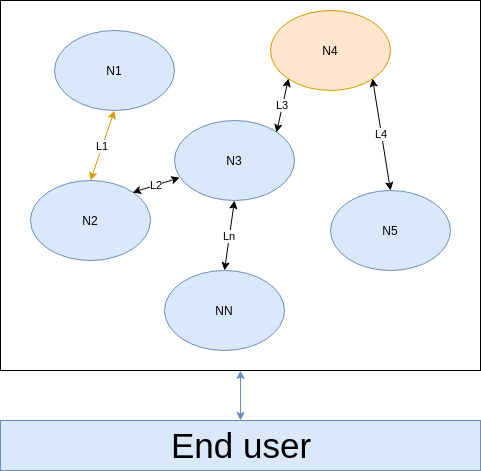
\includegraphics[width=0.7\linewidth]{../img/distributed-system.png}
      \end{figure}
    \end{columns}
  \end{frame}




  \begin{frame}{Introduction}
    \framesubtitle{Distributed systems}
      The desired properties of a distributed system are the following:\vspace{10pt}
      \begin{itemize}
        \item \textbf{Consistency}: all the nodes have the same lates available copy of the data.
        \item \textbf{Availability}: the system is always working and responding to the
        input requests without any failures.
        \item \textbf{Partition tolerance}: if a group of nodes fails the distributed system
        still continues to operate correctly
      \end{itemize}
  \end{frame}




  \begin{frame}{Introduction}
    \framesubtitle{Distributed systems}
    Even if some of the nodes fault or links break, a distributed system should tolerate
    this and should continue to work correctly. There are two types of fault:
    \begin{itemize}
      \item Simple node crash
      \item Exhibition of malicious or inconsistent behavior arbitrarily: \red{Byzantine fault}
    \end{itemize}

    \pause 
    \begin{block}{Byzantine nodes}
      A \textcolor{red}{Byzantine node} is a node that has an arbitrary behavior,
      which can even be malicious.
    \end{block}
  \end{frame}




  \begin{frame}{Introduction}
    \framesubtitle{Distributed systems}
    \begin{block}{Consensus}
      \red{Consensus} is the process of agreement between untrusted nodes on a data
      value.
    \end{block}

    \pause
    Requirements for a consensus algorithm:
    \begin{itemize}
      \item \textbf{Agreement}: non-byzantine nodes must agree on the same value
      \item \textbf{Termination}: the consensus process must come to an end (nodes
      have to reach a decision)
      \item \textbf{Validity}: the agreed value must have been proposed by at
      least one honest node
      \item \textbf{Fault tolerance}: the consensus algorithm must work even
      in the presence of one or more Byzantine nodes
    \end{itemize}
  \end{frame}



  \begin{frame}{Introduction}
    \framesubtitle{Distributed systems}
        \begin{block}{The Byzantine generals problem}
          \begin{itemize}
            \item Problem formulated by Leslie Lamport \cite{lamport1982byzantine}
            \item A group of generals are surrounding a city and they have to agree
            on a common decision: attack or retreat.
            \item Their only communication way is a messenger
            \item Some of the generals may be \emph{traitors}: they communicate
            misleading message for preventing the loyal generals from reaching an
            agreement
            \item Requirement: algorithm that allows the loyal generals to agree
            on the same plan regardless of traitors general
          \end{itemize}
        \end{block}
\end{frame}

\begin{frame}{Introduction}
    \framesubtitle{Distributed system}
    \begin{figure}[!htb]
            \centering
            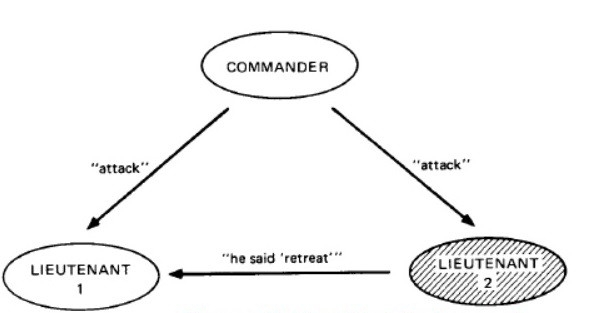
\includegraphics[width=0.5\linewidth]{../img/byzantine.jpg}
    \end{figure}
    \begin{figure}
        \centering
        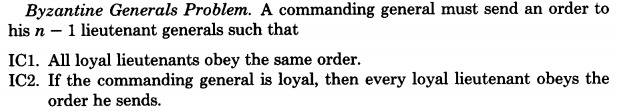
\includegraphics[width=0.7\linewidth]{../img/byzantine-generals-problem.png}
    \end{figure}
\end{frame}






  %%%%%%%%%%%%%%%%%%%%%
  %%% SECOND SECTION %%%
  %%%%%%%%%%%%%%%%%%%%%
  \section{Introduction to Blockchain}
  \subsection{Definition}

  \begin{frame}{What is Blockchain}
    \begin{block}{Business definition}
      Blockchain is a platform whereby peers can exchange values without the need
      for a central trusted party by using transactions which are stored inside
      the platform in a verifiable and permanent way.
    \end{block}
    
    \pause
    \begin{block}{Technical definition}
      Blockchain is a distributed ledger that is
      \begin{itemize}
        \item cryptographically secure
        \item append-only
        \item immutable (extremely hard to change)
        \item updateable only via consensus among nodes
      \end{itemize}
    \end{block}
  \end{frame}



  \subsection{Features}
  \begin{frame}{Blockchain features}
    \begin{itemize}
      \item \textbf{Decentralization}: no need of a central trusted entity
      which stores the data and validates the transaction \pause
      \item \textbf{Distributed consensus}: high Byzantine Fault
      Tolerance, for each data value there's only a single version agreed by all
      parties through a consensus algorithm \pause
      \item \textbf{High availability}: Blockchain is based on a peer-to-peer
      network and data replicated on each node: even if one or more nodes fail
      the whole network can continue to work correctly
    \end{itemize}
  \end{frame}

  \begin{frame}{Blockchain features (Cont.)}
    \begin{itemize}
      \item \textbf{Immutability}: once a block has been added to the blockchain,
      changing it is computationally infeasible \pause
      \item \textbf{Transparency}: every node can see what is in the blockchain \pause
      \item \textbf{Security}: integrity of data, authentication and non-repudiation
      are ensured. Confidentiality is not provided. Security is a consequence of
      the distributed nature of Blockchain \pause
      \item \textbf{Uniqueness}: every transaction is unique and has not been spent already
    \end{itemize}
  \end{frame}



  \subsection{Structure}
  \begin{frame}{Blockchain structure}
    \begin{itemize}
      \item Linked list of ordered fixed-length \red{blocks}
      \item Each block includes a set of \red{transactions}
    \end{itemize}

    \begin{figure}[!htb]
      \centering
      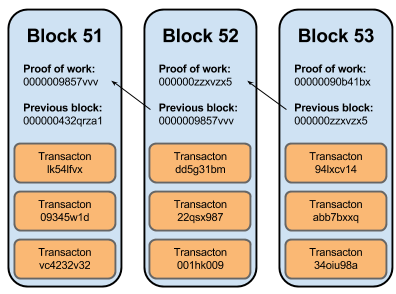
\includegraphics[width=0.45\linewidth]{../img/blockchain-basic-schema.png}
    \end{figure}
  \end{frame}




  \begin{frame}{Blockchain structure}
    \framesubtitle{Blocks structure}
      \begin{itemize}
        \item  A block is a group of transactions. Generally, it is composed of:
        \begin{itemize}
          \item[-] a set of transactions
          \item[-] a hash which identifies the block
          \item[-] a pointer to the previous block hash
          \item[-] a nonce
          \item[-] a timestamp
        \end{itemize}
        \item The first block in the blockchain is called \red{genesis block}.
      \end{itemize}
  \end{frame}




  \begin{frame}{Blockchain structure}
    \framesubtitle{Nodes, addresses and transactions}
    \begin{itemize}
      \item \textbf{Nodes} are active entities which store a copy of the blockchain and can
      perform and/or validate transactions \pause
      \item \textbf{Addresses} are unique identifiers which identify the parties involved in a
      transaction and usually are a public key or are derived from a public key. \pause
      \item \textbf{Transactions} are transfers of value from an address to another. \pause
      \item \textbf{Transaction scripts} are predefined sets of commands for nodes to transfer
      values from one address to another and perform various other functions.
    \end{itemize}
  \end{frame}



  \subsection{Consensus}
  \begin{frame}{Consensus in Blockchain}
      \begin{itemize}
        \item Required to establish whether the ledger itself or new blocks are
        valid or not
        \item Analogy with the Byzantine Generals Problem: ``generals'' are the nodes of the Blockchain, ``messengers'' are the network links and ``traitors'' are malicious nodes which try to tamper with the data
      \end{itemize}
  \end{frame}
  
  
  
  \begin{frame}{Consensus in Blockchain}
      Consensus mechanisms commonly used in Blockchain:
      \begin{enumerate}
        \item Practical Byzantine Fault Tolerance (\textbf{PBFT})
        \item Proof of Work (\textbf{PoW})
        \item Proof of Stake (\textbf{PoS})
        \item Delegated Proof of Stake (\textbf{DPoS})
      \end{enumerate}
  \end{frame}




  \begin{frame}{Consensus in Blockchain}
    \framesubtitle{Common Consensus mechanisms}
    \begin{block}{1) Practical Byzantine Fault Tolerance}
      \begin{itemize}
        \item Algorithm proposed by M. Castro and B. Liskov as an optimized
        solution to the Byzantine Generals Problem \cite{castro1999practical} 
        \item Each “general” maintains an internal state. When he receives a
        message, he uses it in conjunction with his internal state to
        run a computation which tells what to think about the message in question 
        \item  After reaching his individual decision about the message,
        the general shares that decision with all the other “generals” in the system 
        \item  A consensus decision is determined based on the total decisions
        submitted by all generals \pause
        \item \textcolor{green}{Pro}: very efficient \pause
        \item \red{Cons}: precludes users anonimity \pause
        \item Mechanism adopted by Hyperledger and Ripple
      \end{itemize}
    \end{block}
  \end{frame}




  \begin{frame}{Consensus in Blockchain}
    \framesubtitle{Common Consensus mechanisms}
    \begin{block}{2) Proof of Work}
      \begin{itemize}
        \item Contrary to the PBFT, it doesn’t require all nodes to submit
        their individual conclusions 
        \item Based on a proof that ensures that enough computational resources have
        been spent before proposing a block for acceptance by the network 
        \item Only a single node (the first one who solves the PoW) announces its
        block 
        \item The announced blocks can be independently verified by all
        the nodes in the system \pause
        \item Mechanism adopted by Bitcoin
      \end{itemize}
    \end{block}
  \end{frame}





  \begin{frame}{Consensus in Blockchain}
    \framesubtitle{Common Consensus mechanisms}
    \begin{block}{3) Proof of Stake}
      \begin{itemize}
        \item Contrary to PoW, there isn't any individual attempting to carry out
        an intensive computation in order to propose a block 
        \item The network runs a lottery based on the nodes’ stake to decide
        who will announce a block 
        \item The more stake one node has, the higher the probability
        to be chosen is 
        \item \textcolor{green}{Main idea}: if a node that has enough stake in the system it means
        that it has invested enough in the system \MVRightarrow\, any malicious
        attempt/attack on the system wouldn't have any benefits for him \pause
        \item \red{Main problem}: the system rewards more those who already are most
        deeply involved in the network \MVRightarrow\, the system becomes always
        more centralized
      \end{itemize}
    \end{block}
  \end{frame}





  \begin{frame}{Consensus in Blockchain}
    \framesubtitle{Common Consensus mechanisms}
    \begin{block}{4) Delegated Proof of Stake}
      \begin{itemize}
        \item Evolution of the PoS 
        \item Each node that has stake in the system can choose an entity to
        represent its portion of stake in the system (by voting) 
        \item The more stake one node has, the higher is the weight of his vote 
        \item The entity with most votes (weighted) becomes a delegate which
        proposes blocks 
        \item The voting process is periodically executed: if the current delegate
        doesn't behave correctly the other nodes just stop voting it
      \end{itemize}
    \end{block}
  \end{frame}



  \subsection{Types of Blockchain}
  \begin{frame}{Types of Blockchain}
    \begin{block}{1) Public Blockchain}
      \begin{itemize}
        \item Blockchain open to the public in which everyone can join the network,
        maintain the shared ledger and participate in the consensus process 
        \item The ledger is not owned by anyone and everyone can read it 
        \item Usually there's an incentive mechanism to encourage more participants
        to join the network \pause
        \item \red{Main problem}: lack of privacy (everyone can see the transactions
        stored in the blockchain) \pause
        \item Bitcoin is based on a public blockchain
      \end{itemize}
    \end{block}
  \end{frame}




  \begin{frame}{Types of Blockchain (Cont. 1)}
    \begin{block}{2) Private Blockchain}
      \begin{itemize}
        \item Open only to an organization or a group of individuals
        \item Participants need to obtain an invitation or permission to join the Blockchain and maintain the ledger
        \item Usually the network is permissioned: restrictions on who is allowed to participate in the network and only in certain transactions 
        \item Example of private Blockchain: Hyperledger Fabric \cite{hyperledger-fabric}
      \end{itemize}
    \end{block}
  \end{frame}




  \begin{frame}{Types of Blockchain (Cont. 2)}
    \begin{block}{3) Consortium Blockchain}
      \begin{itemize}
        \item Consensus process is controlled by a preselected set of nodes (e.g. a consortium of organizations, each of which operates a node) 
        \item The right to read the blockchain might be public or permissioned 
        \item Example of consortium Blockchain: R3 \cite{R3}
      \end{itemize}
    \end{block}
  \end{frame}










  %%%%%%%%%%%%%%%%%%%%%
  %%% THIRD SECTION %%%
  %%%%%%%%%%%%%%%%%%%%%
  \section{Bitcoin}
  \subsection{What is Bitcoin}
  \begin{frame}{What is Bitcoin}
    \begin{itemize}
      \item First fully decentralized cryptocurrency 
      \item Invented by Satoshi Nakamoto in 2008: first real implementation of
      Blockchain 
      \item Bitcoin can be either defined as a protocol, a digital currency
      and a platform: 
      \begin{itemize}
        \item Bitcoin (capital B)  \MVRightarrow\, Bitcoin protocol
        \item bitcoin (lowercase b) \MVRightarrow\, bitcoin  currency
      \end{itemize} \pause
    \end{itemize}

    \begin{block}{The reference implementation}
      \begin{itemize}
        \item Bitcoin is an open source project and is developed by a community of volunteers
        \item The reference implementation is \textbf{Bitcoin Core}
        \item It is considered the authoritative implementation and it specifies
        how each part of the system has to be implemented.
      \end{itemize}
    \end{block}
  \end{frame}




  \begin{frame}{What is Bitcoin (Cont. 1)}
    Bitcoin can be seen as a combination of:
    \begin{itemize}
      \item a decentralized peer-to-peer-network (the Bitcoin protocol)
      \item a public transaction ledger (the blockchain) 
      \item a set of rules for validating transactions (consensus rules) 
      \item a mechanism for reaching distributed consensus on the blockchain
      (distributed consensus algorithm) 
    \end{itemize}
  \end{frame}





  \begin{frame}{What is Bitcoin (Cont. 2)}
    Bitcoins are entirely ``virtual'':
    \begin{itemize}
      \item there aren't any physical or virtual coins stored anywhere 
      \item the coins are implied in the transactions that send value from a sender to
      a receiver
    \end{itemize}
  \end{frame}





  \subsection{Scripts}
  \begin{frame}{Bitcoin scripts}
    \begin{itemize}
      \item Script = list of instructions recorded with each transaction that describes
      how the next person wanting to spend the Bitcoins being transferred can gain access to them \pause 
      \item Programming language used: ``\red{Script}'' \cite{script-bitcoin-wiki} 
      \begin{itemize}
        \item very simple programming language 
        \item not Turing-complete {\tiny(no loops and no complex control flow instructions)} 
        \item deliberately disegned like this for avoiding abuses of the scripts
        for conducting denial of service attacks {\tiny(each scripts has to be
        executed on each node of the network)}
      \end{itemize}
    \end{itemize}
  \end{frame}




  \subsection{Keys and addresses}
  \begin{frame}{Keys and addresses}
    \begin{itemize}
      \item Ownership of bitcoins is established through digital keys, Bitcoin addresses, and digital signatures 
      \item In order to be included in the blockchain, transactions require a valid
      signature which can be generated only with a private (secret) key 
      \item The private key proves the ownership of bitcoins by signing transactions and
      transferring value from a user to another \pause
    \end{itemize}
    \begin{block}{Analogy with traditional banking}
      \begin{itemize}
        \item public key \MVRightarrow\, bank account number
        \item private key \MVRightarrow\, secret PIN (or signature on a check)
        which which allows to unlock the value and transferring it to other people
      \end{itemize}
    \end{block}
  \end{frame}





  \begin{frame}{Keys and addresses (Cont. 1)}
    \begin{block}{Addresses}
      \begin{itemize}
        \item unique strings of digits and characters which identify the originator and/or the destination of a transaction \pause
        \item derived from public keys through one-way cryptographic hashing:
        \begin{enumerate}
          \item Double hashing: SHA-256 + RIPEMD160
          \item 160-bit hash as result
          \item Base58Check encoding of the 160-bit hash
          \item Result: 26-35 characters string which begins with “1” (\red{public key
          address}) or “3” (\red{pay-to-script-hash address})
        \end{enumerate}
      \end{itemize}
    \end{block}
  \end{frame}





  \begin{frame}{Keys and addresses (Cont. 2)}
    \begin{block}{Keys}
      \begin{itemize}
        \item Private keys are 256-bit random numbers and can be represented
        in different formats \pause
        \item Public keys are generated starting from the private keys using
        elliptic curve multiplication: \pause
        \begin{itemize}
          \item ``Trap door'' function 
          \item Elliptic curve  specified by the secp256k1 standard, defined by the NIST:
          \[ y^2 \bmod p = (x^3 + 7) \bmod p \]
          where $p = 2^{256} – 2^{32} – 2^9 – 2^8 – 2^7 – 2^6 – 2^4 – 1$ is a very large prime number 
          \item Public key $K=k*G$, where $k$ is the private key and $G$ is
          a point on the curve defined by the standard 
          \item The generator point $G$ is always the same for all Bitcoin users
        \end{itemize}
      \end{itemize}
    \end{block}
  \end{frame}





  \begin{frame}{Keys and addresses (Cont. 3)}
    \begin{block}{Public key formats}
      \begin{itemize}
        \item \textbf{Uncompressed format}: the key is the coordinates pair
        $(x,y)$ of a point on the curve \MVRightarrow\, prefix $04$ followed by
        two 256-bit numbers (65 Bytes) \pause
        \item \textbf{Compressed format}: prefix $03$ (if the y-coordinate is an
        odd number) or $02$ (if the y-coordinate is an even number) followed
        by the x-coordinate \MVRightarrow\ 33 Bytes.
        \begin{itemize}
          \item the y-coordinate can be derived from the x one \pause
        \end{itemize}
        \item Address derived from a compressed public key $\neq$ address derived
        from the uncompressed version \pause
        \begin{itemize}
          \item solution: \textbf{compressed private keys}
          \item private keys from which only compressed
          public keys should be derived
        \end{itemize}
      \end{itemize}
    \end{block}
  \end{frame}




  \subsection{Transactions}
  \begin{frame}{Transactions}
    \begin{itemize}
      \item Data structures that encode the transfer of value between participants
      in the bitcoin system 
      \item They're public visible by anyone 
      \item A transaction includes at least one input and output
    \end{itemize}
  \end{frame}





  \begin{frame}{Transactions (Cont. 1)}
    \begin{block}{Transaction outputs}
      \begin{itemize}
        \item Discrete and indivisible units of bitcoin measured in Satoshi 
        \item Can be seen as coins being created in a transaction \pause 
        \item Consist of two parts:
        \begin{enumerate}
          \item amount of bitcoin (expressed in Satoshi)
          \item set of conditions required for spending the output (\textbf{locking script})
        \end{enumerate}
        \pause
        \item All the available and spendable outputs are stored in the blockchain
        and they are called unspent transaction outputs or (\textbf{UTXO}) 
        \item Balance shown by Wallets application is the aggregated value of
        all the UTXOs the user can spend with the keys it controls 
        \item UXTO can only be spent in its entirety by a transaction \pause
        \begin{itemize}
          \item[$\rightarrow$] usually transactions generate \emph{change}
        \end{itemize}
      \end{itemize}
    \end{block}
  \end{frame}





  \begin{frame}{Transactions (Cont. 2)}
    \begin{block}{Transaction inputs}
      A transaction input consists of: 
      \begin{enumerate}
        \item one or more UTXOs that will be consumed 
        \item a proof of ownership through the locking script to unlock the selected UXTO \pause
        \begin{itemize}
          \item[$\rightarrow$] usually consists of a digital signature and a public key
        \end{itemize}
      \end{enumerate}
    \end{block}
  \end{frame}





  \begin{frame}{Transactions (Cont. 3)}
    \begin{block}{Transaction typical life cycle}
      \begin{enumerate}
        \item A sender sends a transaction (using a wallet application) 
        \item The wallet signs the transaction using the sender’s private key in order
        to prove the ownership of the value being transferred 
        \item The transaction is broadcasted to the Bitcoin network 
        \item Mining nodes include this transaction in the next block to be mined 
        \item When a node solves the Proof of Work it broadcasts the
        newly block to the network 
        \item Confirmation process starts: each node verifies the new block and propagate it further
      \end{enumerate}
    \end{block}
  \end{frame}




  \begin{frame}{Transactions (Cont. 4)}
    \begin{block}{Transaction fees}
      \begin{itemize}
        \item Two purposes:
        \begin{enumerate}
          \item Compensate the miners 
          \item Act as a security mechanism: economically infeasible for attackers to flood the network with transactions 
        \end{enumerate}
        \item Their value depends on the size of the transaction:
        \[ Fees = Sum(Inputs)–Sum(Outputs) \] 
        \item The spender is the one that decides how much fee to pay
        \begin{itemize}
            \item the miners choose from a pool the transactions to include in the next block
            \item higher fee = faster confirmation (mined quicker)
            \item null fee = the transaction will likely never be mined
        \end{itemize}
      \end{itemize}
    \end{block}
  \end{frame}





  \begin{frame}{Transactions (Cont. 5)}
    \begin{block}{Coinbase transactions}
      \begin{itemize}
        \item First transaction in a block 
        \item Created by the first node which solves the proof-of-work 
        \item Create brand-new bitcoins that the miner can spend as a reward for mining
        \item Do not consume UTXO: they have special type of input called coinbase
      \end{itemize}
    \end{block}
  \end{frame}





  \subsection{Wallets}
  \begin{frame}{Wallets}
    \begin{itemize}
      \item Applications that serve as a user interface and manage user’s money 
      \item Technically: data structures that securely store the user’s private keys required for spending the bitcoins he possesses 
      \item They don't store ``money'' but only pairs of public/private keys
      \item Two kind of wallets: \emph{deterministic} and \emph{nondeterministic}
    \end{itemize}
  \end{frame}




  \begin{frame}{Wallets (Cont. 1)}
    \begin{block}{Nondeterministic wallets}
      \begin{itemize}
        \item Each key is independently generated starting from a random number \MVRightarrow\, keys stored in the wallet are not related to each other \
        \item Main disadvantage: cumbersome to manage 
        \begin{itemize}
          \item[-] they have to be backed up frequently \MVRightarrow\, each key has to be backed up 
          \item[-] address reuse avoidance \MVRightarrow\, many addresses \MVRightarrow\, many keys that has to be backed up frequently
        \end{itemize}
      \end{itemize}
    \end{block}
  \end{frame}




  \begin{frame}{Wallets (Cont. 2)}
    \begin{block}{Deterministic wallets}
      \begin{itemize}
        \item All the keys are derived from a single master key (the \emph{seed}) 
        \item The stored keys can be generated again if one has the original seed 
        \item Only the seed has to be backed up 
        \item Easily manageable, even if using address reuse avoidance 
        \item Keys usually derived in a tree structure (BIP-32 standard) 
        \begin{itemize}
            \item high flexibility
        \end{itemize}
        \item Seeds usually created according to BIP-39 standard 
        \begin{itemize}
          \item[-] sequence of English words called \emph{mnemonic} 
          \item[-] easy to transcribe, export and import across wallets
        \end{itemize}
      \end{itemize}
    \end{block}
  \end{frame}




  \subsection{Bitcoin Blockchain}
  \begin{frame}{Bitcoin Blockchain}
     \begin{itemize}
         \item Linked list of blocks of transactions
         \item Each block is identified by a SHA-256 hash
         \item Each blocks embeds in its header the hash of the previous block
         \begin{itemize}
             \item changing a block causes its hash to change
             \item the hash of the children blocks changes as well (cascade effect)
         \end{itemize}
         \item Once a block has enough children, it cannot be changed without recalculating all the subsequent blocks
         \begin{itemize}
             \item[\MVRightarrow] blockchain history is practically immutable
         \end{itemize}
     \end{itemize}
  \end{frame}
  
  
  
  \begin{frame}{Bitcoin Blockchain}
    \begin{figure}[!htb]
    \centering
    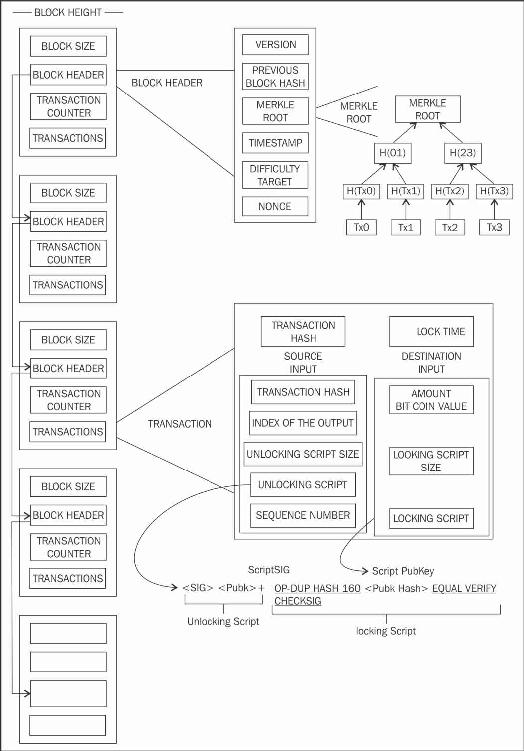
\includegraphics[width=0.45\linewidth]{../img/bitcoin-blockchain-scheme.png}
    \end{figure}
  \end{frame}
  
  
  
  \begin{frame}{Bitcoin Blockchain}
      \begin{block}{Merkle Trees}
          \begin{itemize}
              \item Data structure used for summarize and verify the integrity of large sets of data in an efficient way (Binary tree of hashes)
              \item Used for efficiently verify if a transaction is included in a block
              \item The root of the tree stored in each block summarizes all the transactions included in that block
              \begin{itemize}
                  \item [\MVRightarrow] nodes can verify transactions without downloading all the block transactions (but just a Merkle path + block header)
              \end{itemize} 
          \end{itemize}
      \end{block}
  \end{frame}
  
  
  
  \begin{frame}{Bitcoin Blockchain}
    \framesubtitle{Merkle Trees}
    \begin{figure}
      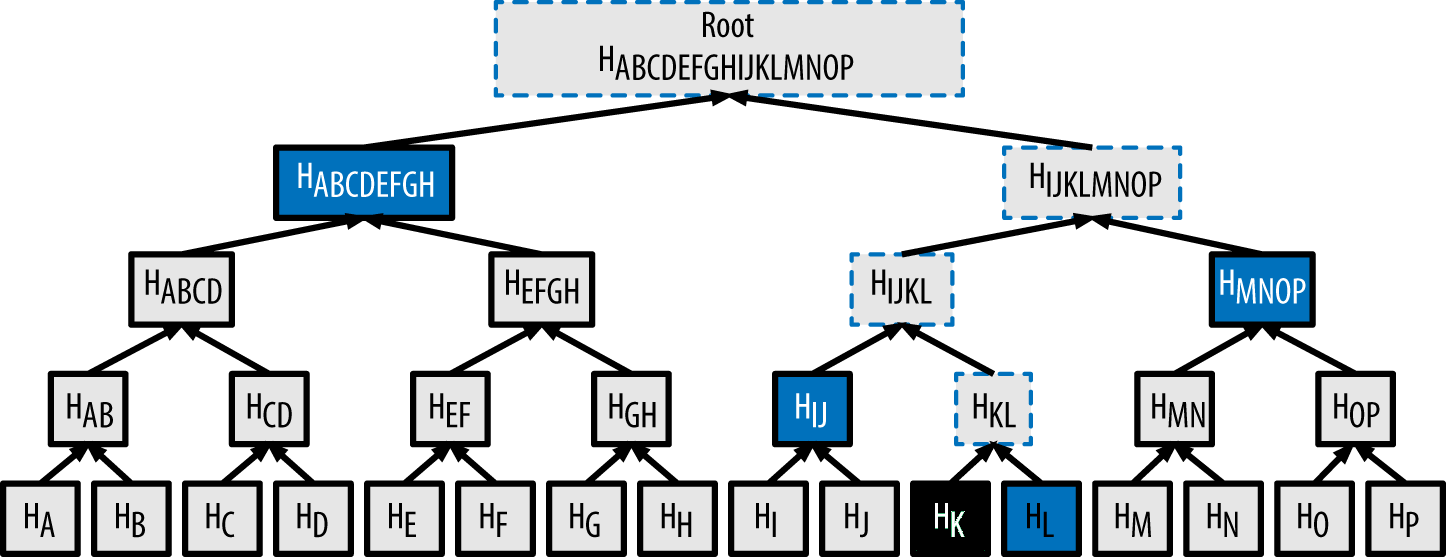
\includegraphics[width=0.6\linewidth]{../img/merkle-tree-path.png}
    \end{figure}
    \begin{itemize}
        \item To check if a transaction is included in a block, only $log_2(N)$ hashes have to be downloaded ($N$ number of transactions of the block)
    \end{itemize}
  \end{frame}
  
  
  
  
  
  \begin{frame}{Bitcoin Blockchain}
  \framesubtitle{Merkle Trees}
      \footnotesize
       \begin{tabularx}{\textwidth}{l l l l}
         \toprule
         \textbf{Number of transactions}	& \textbf{Approx size of block} & \textbf{Path size} &	\textbf{Path size}   \\ \midrule
         16 transactions & 4 kilobytes & 4 hashes & 128 bytes \\
         \\
         512 transactions & 128 kilobytes & 9 hashes & 288 bytes \\
         \\
         2048 transactions & 512 kilobytes & 11 hashes & 352 bytes \\
         \\
         65535 transactions & 16 megabytes & 16 hashes & 512 bytes \\
         \bottomrule
     \end{tabularx}
  \end{frame}
  
  
  
  
  \subsection{Bitcoin Network}
  \begin{frame}{Bitcoin Network}
    The network is a peer-to-peer network
    \begin{itemize}
        \item no ``special'' nodes (all the nodes consume and provide services) 
        \item flat network topology
        \item nodes connected in a mesh
    \end{itemize}
    
    Three different types of nodes:
    \begin{enumerate}
        \item Full nodes
        \item Miners
        \item Lightweight clients
    \end{enumerate}
    
    Despite the type, all the nodes validate and propagate transactions (blocks)
  \end{frame}
  
  
  
  
  \begin{frame}{Bitcoin Network}
    \framesubtitle{Node types}
    \begin{block}{1) Full nodes}
        \begin{itemize}
            \item Maintain a full copy of the Blockchain
            \begin{itemize}
                \item[\MVRightarrow] they can autonomously and authoritatively verify transactions
            \end{itemize}
            \item Validate and forward transactions/blocks to their peers 
            \item Drawback: the size of the Blockchain is currently around 178 GB \cite{statista}
        \end{itemize}
    \end{block}
  \end{frame}
  
  
  
  
   \begin{frame}{Bitcoin Network}
    \framesubtitle{Node types}
    \begin{block}{2) Miners}
        \begin{itemize}
            \item Nodes that solve the proof-of-work and create new blocks
            \item They compete with each other
            \item They do not necessarily have to be full-nodes
            \begin{itemize}
                \item[\MVRightarrow] they participate to mining pools \footnote{Mining pool = groups of cooperating miners who agree to share block rewards in proportion to their contributed mining hash power} in which a pool server maintain the full copy of the Blockchain
            \end{itemize}
        \end{itemize}
    \end{block}
  \end{frame}
  
  
  
  
  \begin{frame}{Bitcoin Network}
    \framesubtitle{Node types}
    \begin{block}{3) Lightweight clients}
        \begin{itemize}
            \item Clients designed to run on limited resources devices (e.g. smartphones, tablets, etc.) 
            \item They store only the headers of the blocks 
            \item They validate transactions using a Simple Payment Verification (SPV) scheme \footnote{e.g. they have to verify that none of the transaction's inputs have been previously spent}
            \begin{itemize}
                \item[-] they check if a transaction belongs to a block by requesting a Merkle Path to a full node
                \item[-] they validate the proof-of-work of the block
                \item[-] they do not build the UTXO set: they check how deep the block of the transaction is ``buried'' \MVRightarrow many blocks above it = the transaction is valid (e.g. it's not double-spent)
            \end{itemize}
        \end{itemize}
    \end{block}
  \end{frame}





  \begin{frame}{References}
    \printbibliography
  \end{frame}

\end{document}
